% -------------------------------------------------------------------------------------- %

\section{Numerical Methods}

\subsection{Petrov-Galerkin Methods}

The original Ritz-Galerkin method is described as follows: we are given a PDE problem in 
its \emph{weak formulation}: 
\begin{equation}
    \label{eq:weak_pde}
    \text{find } u \in \scrX \text{ such that } q(v, u) 
    = \left\langle f, v \right\rangle\ \forall\; v \in \scrW
\end{equation}
where $q$ is some elliptic sesquilinear form, $f \in \scrX$ given, 
$\left\langle \cdot, \cdot \right\rangle$ some inner product, and $\scrW$ some 
\emph{test set}. The form $q$ is typically derived from some minimization problem for a 
functional representing energy. 

The idea behind the Ritz-Galerkin method is to \emph{solve \ref{eq:weak_pde} on a 
finite-dimensional subspace:} let 
$\scrW = \spn \left\{ \psi_1, \ldots, \psi_N \right\}$ be 
$q$-linearly independent. 

Then writing 
\begin{equation}
    \label{eq:Psi}
    \Psi (x) = \left[ \psi_1 (x) \mid \ldots \mid \psi_N (x) \right] , 
\end{equation}
we make the 
approximation $u \approx \Psi c_u$ and have $v = \Psi c_v$ for $c_u, c_v \in \bbC^N$. 
Now \ref{eq:weak_pde} reduces to 
\begin{equation}
    \text{find } c_u \in \bbC^N \text{ such that } 
    q( \Psi c_v, \Psi c_u )
    = \left\langle f, \Psi c_v \right\rangle\ \forall\; c_v \in \bbC^N . 
\end{equation}
One quickly verifies that $c_u$ is the unique solution to the matrix equation $A x = b$ 
with 
\begin{equation}
    A_{i j} = q( \Psi e_i, \Psi e_j ) = q( \psi_i, \psi_j ), \quad
    b_i = \left\langle f, \Psi e_i \right\rangle 
    = \left\langle f, \psi_i \right\rangle . 
\end{equation}
where $e_i \in \bbC^N$ is the $i$-th standard unit vector. $A$ is known as the 
\emph{stiffness matrix}. 

One can extend the Ritz-Galerkin formulation by allowing the test space to differ from 
the basis space: keep $u \approx \Psi c_u$ but let 
$\scrW = \spn \left\{ \psi^*_1, \ldots, \psi^*_M \right\}$, then $A$ and $b$ become 
\begin{equation}
    A_{i j} = q( \psi^*_i, \psi_j ), \quad 
    b_i = \left\langle f, \psi^*_i \right\rangle . 
\end{equation}
In the regime $M > N$ this equation is \emph{overdetermined} so it is solved in a least 
squares sense
\begin{equation}
    \left\| A x - b \right\|_2^2 = \min_{x \in \bbC^N} !
\end{equation}
where $\left\| \cdot \right\|_2$ is the vector $\ell^2$ norm. This is known as the 
Petrov-Galerkin method. 

One can extend the method further by asking that multiple solutions for multiple right 
hand sides $(f_j)_{j=1}^N$ are computed simultaneously, that is 
\begin{equation}
    \label{eq:galerkin}
    \left\| A X - B \right\|_F^2 = \min_{X \in \bbC^{N \times N}} !, \quad 
    B_{i j} = \left\langle f_j, \psi^*_i \right\rangle 
\end{equation}
where $\left\| \cdot \right\|_F$ denotes the Frobenius norm. 

Numerically, \ref{eq:galerkin} can be solved using the Moore-Penrose inverse
\begin{equation}
    \label{eq:moore_penrose}
    X = A^\dagger B . 
\end{equation}
An exercise in matrix calculus shows that the solution can also be written in the form 
\begin{equation}
    \label{eq:adjoint_inverse}
    X = (A^* A)^{-1} A^* B . 
\end{equation}
Both forms will prove to be useful later. 


\subsection{Extended Dynamic Mode Decomposition (EDMD)}

\subsubsection{The Galerkin Ansatz}

We apply the Petrov-Galerkin Ansatz to obtain a matrix approximation $K$ 
for $\left. \scrK \right|_{\scrX}$. Let 
$q(\cdot, \cdot) = \left\langle \cdot, \cdot \right\rangle$ and consider a linearly 
independent family of functions $\left\{ \psi_1, \ldots, \psi_N \right\} \subset \scrX$. 
Take delta distributions, that is $\left\langle \delta_x, \psi \right\rangle = \psi (x)$, 
for the test function(als): let $(w_i, x_i)_{i=1}^M$ represent a quadrature scheme and 
set $\psi_i^* = \sqrt{w_i} \delta_{x_i}$. 

We then solve the Galerkin equation \ref{eq:galerkin} for $f_j = \scrK \psi_j$: 
\begin{equation}
    \label{eq:edmd}
    \left\| \sqrt{W} \YX K - \sqrt{W} \YY \right\|_F^2 = \min_{K \in \bbC^{N \times N}} !
\end{equation}
with $W = \diag (w_1, \ldots, w_M)$ and 
\begin{equation}
    (\YX)_{i j} = \left\langle \delta_{x_i}, \psi_j \right\rangle = \psi_j (x_i), \quad
    (\YY)_{i j} = \left\langle \delta_{x_i}, \scrK \psi_j \right\rangle = \psi_j (\, S (x_i) \,) . 
\end{equation}

This results in the \emph{EDMD matrix} $K = \YX^\dagger \YY = (\YX^* W \YX)^{-1} (\YX^* W \YY)$. 
Inverting $\YX$ involves computing the Moore-Penrose inverse of an $N \times M$ matrix, 
whereas inverting $\YX^* \YX$ involves computing the inverse of a symmetric $N \times N$ 
matrix. Depending on the relationship between $M$ and $N$ in the particular usecase, 
either forumlation might be cheaper. 

Another look at the second formulation of the EDMD matrix shows that 
\begin{equation}
    \label{eq:G}
    G_{i j} \defeq 
    ( \YX^* W \YX )_{i j} 
    = \sum_{k=1}^{M} w_k \overline{\psi_i (x_k)} \psi_j (x_k)
    \xrightarrow{\makebox[1.2cm]{\scriptsize{M \to \infty}}} 
    \left\langle \psi_i, \psi_j \right\rangle 
    \eqdef \bbG_{i j} , 
\end{equation}
\begin{equation}
    \label{eq:A}
    A_{i j} \defeq
    ( \YX^* W \YY )_{i j} = \sum_{k=1}^{M} w_k \overline{\psi_i (x_k)} \psi_j (\, S(x_k) \,)
    \xrightarrow{\makebox[1.2cm]{\scriptsize{M \to \infty}}} 
    \left\langle \psi_i, \scrK \psi_j \right\rangle
    \eqdef \bbA_{i j} , 
\end{equation}
which can be computed with constant memory requirement. 

\subsubsection{Functional Minimization}\label{sec:functional_minimization}

We could have arrived at equation \ref{eq:edmd} completely differently: 
equation \ref{eq:edmd} is precisely a quadrature approximation of the functional least 
squares minimization:
\begin{equation}
    \label{eq:edmd_functional}
    \left\| \Psi K - \scrK \Psi \right\|_{\scrX^{1 \times N}}^2 
    = \min_{K \in \bbC^{N \times N}} !
\end{equation}
where $\scrK \Psi$ is understood elementwise and
$\scrX^{1 \times N}$ is the space of (row) vector-valued functions with each 
component in $\scrX$
\begin{equation}
    \left\| \left[ f_1 \mid \ldots \mid f_N \right] \right\|_{\scrX^{1 \times N}}^2
    = \left\| f_1 \right\|_{\scrX}^2 + \ldots + \left\| f_N \right\|_{\scrX}^2 . 
\end{equation}

Let us investigate $\Psi : \bbC^N \to \scrX$ a bit closer. Decompose the Hilbert space 
$\scrX$ into 
\begin{equation}
    \scrX = \spn \left\{ \psi_j \right\}_{j=1}^N \oplus \scrV, \quad 
    \scrV = \left( \left\{ \psi_j \right\}_{j=1}^N \right)^\perp
\end{equation}
and let $\left\{ \psi_j \right\}_{j=N+1}^\infty$ be a basis of $\scrV$. 

A short calculation using the orthogonality of $\left\{ \psi_j \right\}_{j=1}^N$ and 
$\left\{ \psi_j \right\}_{j=N+1}^\infty$ shows that for $\phi \in \scrX$, 
\begin{equation}
    \left\langle \phi, \Psi c \right\rangle 
    = \sum_{j=1}^{N} \left\langle \phi, \psi_j \right\rangle c_j . 
\end{equation}
\iffalse
Let $\phi = \sum_{i=1}^{\infty} b_i \psi_i$ and observe
\begin{align}
    \left\langle \phi, \Psi c \right\rangle
    &= \sum_{i=1}^{\infty} \sum_{j=1}^{N} b_i c_j \left\langle \psi_i, \psi_j \right\rangle \\
    &= \sum_{i=1}^{N} \sum_{j=1}^{N} b_i c_j \left\langle \psi_i, \psi_j \right\rangle \\
    &= \sum_{j=1}^{N} \left\langle \sum_{i=1}^{N} b_i \psi_i, \psi_j \right\rangle c_j \\
    &= \sum_{j=1}^{N} \left\langle \sum_{i=1}^{\infty} b_i \psi_i, \psi_j \right\rangle c_j \\
    &= \sum_{j=1}^{N} \left\langle \phi, \psi_j \right\rangle c_j . 
\end{align}
\fi
Hence the adjoint quasi-matrix $\Psi^* : \scrX \to \bbC^N$ acts as 
\begin{equation}
    \Psi^* \phi = \begin{pmatrix}
        \left\langle \phi, \psi_1 \right\rangle \\
        \vdots \\
        \left\langle \phi, \psi_1 \right\rangle
    \end{pmatrix} . 
\end{equation}

\begin{lemma}
    For an arbitrary basis $\left\{ \psi_j \right\}_{j=1}^N$, the orthogonal projector $P$ 
    onto the space spanned by the basis is 
    \begin{equation}
        P = \Psi (\Psi^* \Psi)^{-1} \Psi^* . 
    \end{equation}
\end{lemma}

\begin{proof}
    The solution of a linear least squares problem $\left\| Ax - b \right\| = \min !$ is 
    the result of orthogonally projecting $b$ onto the range of $A$, that is, $A x = P b$. 
    From equation \ref{eq:adjoint_inverse} we know $x = (A^* A)^{-1} A^* b$. Therefore 
    $P b = A x = A (A^* A)^{-1} A^* b$. Since this holds for arbitrary $b$, the result 
    is proven. 
\end{proof}

Using equation \ref{eq:adjoint_inverse} we see that in the infinite-data limit 
$M \to \infty$, $K$ has the form
\begin{equation}
    \label{eq:functional_K}
    K = (\Psi^* \Psi)^{-1} \Psi^* (\scrK \Psi)
\end{equation}
Inserting the definitions of $\Psi$ and $\Psi^*$ yields $K = \bbG^{-1} \bbA$ exactly as 
in equations \ref{eq:G} and \ref{eq:A}. 

If we view the result of applying $K$ as in equation \ref{eq:functional_K} to a vector 
$c$ as an object in $\scrX$, that is, $\Psi K c$, we see that 
\begin{equation}
    \label{eq:PKP}
    \Psi K c = \Psi (\Psi^* \Psi)^{-1} \Psi^* (\scrK \Psi) c
    = P \scrK \Psi c = P \scrK P \Psi c . 
\end{equation}
Since this holds for arbitrary $c$ we have proven that (when viewed as an operator 
on $\scrX$) $K$ is precisely the action of $P \scrK P$, the finite section of $\scrK$ 
over $\spn \left\{ \psi_j \right\}_{j=1}^N$. In this way, EDMD can just as well be viewed 
as a finite section method. 

\begin{algorithm}
    \caption{Extended Dynamic Mode Decomposition (EDMD)}
    \label{alg:edmd}
    \begin{algorithmic}[1]
        \Require Dictionary $\left\{ \psi_j \right\}_{j=1}^N$, data points and weights 
            $\left\{ (w_i, x_i) \right\}_{i=1}^M$
        \State Construct $G$, $A$ as in \ref{eq:G}, \ref{eq:A}
        \State Set $K = G^{-1} A$ (or $L = G^{-1} A^*$)
        \State Compute an eigendecomposition $K V = V \Lambda$ (or $L V = V \Lambda$)
        \State \Return Eigenvalues and eigenmodes $\Lambda$, $V$
    \end{algorithmic}
\end{algorithm}

\begin{figure}
    \centering
    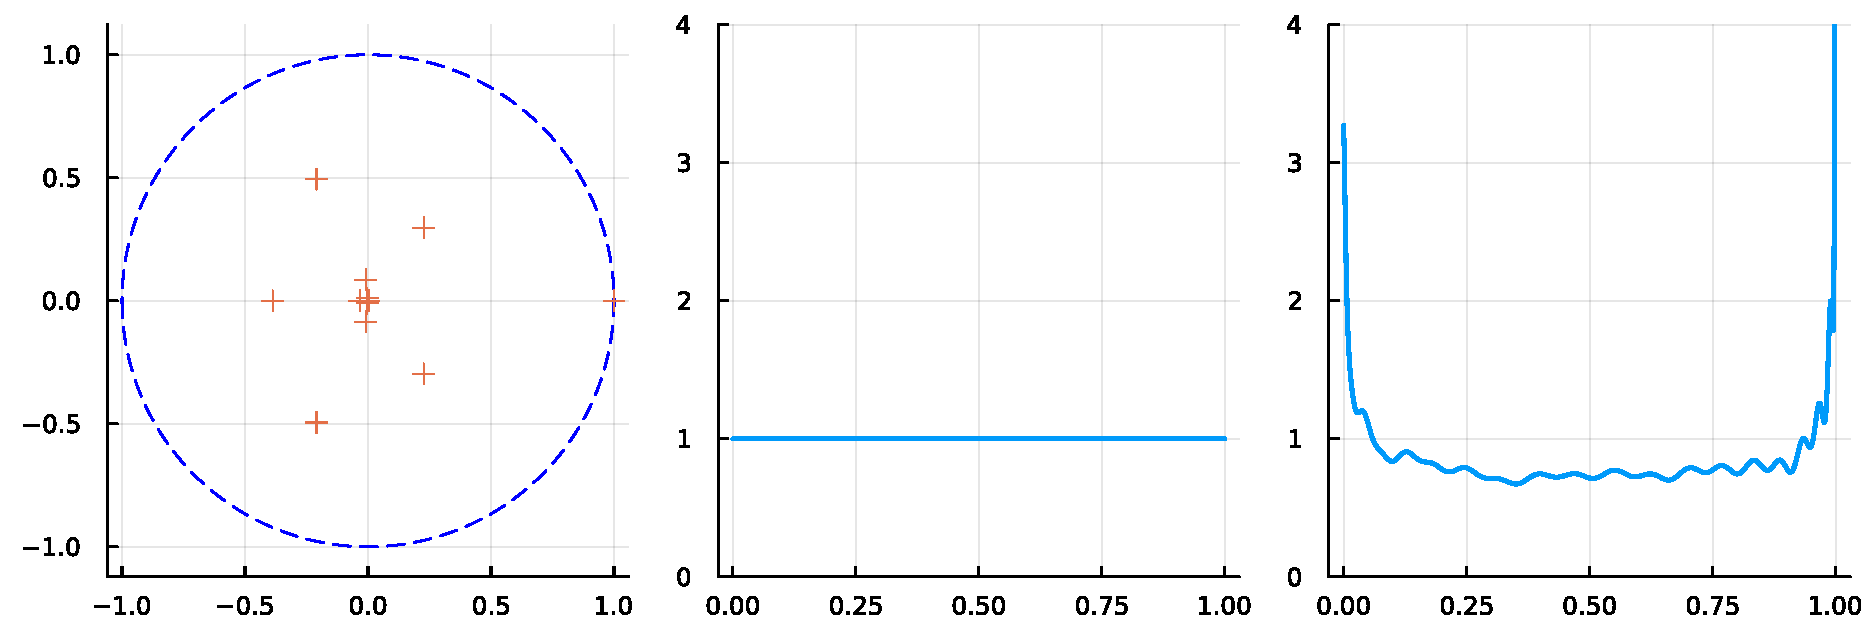
\includegraphics[width=\textwidth]{edmd.pdf}
    \caption{
        Algorithm \ref{alg:edmd} applied to the quadratic map (c.f. figure 
        \ref{fig:perron_asymptotic}) performed with $M = 100$ Gauß-Legendre quadrature 
        nodes and weights, and $N = 40$ Legendre polynomials transplanted to the interval 
        $[0, 1]$. Left: spectrum of $K$. Middle: (normalized) eigenfunction of $K$ for 
        the eigenvalue $\lambda = 1$. Right: (normalized) eigenfunction of $L$ for the 
        eigenvalue $\lambda = 1$. Compare with figure \ref{fig:quadratic_eigs}. 
    }
\end{figure}

\subsubsection{EDMD for the Perron-Frobenius Operator}

From equation \ref{eq:functional_K}, and noting the form of $\bbA$, 
\begin{equation}
    \left\langle \psi_i, \scrL \psi_j \right\rangle 
    = \left\langle \scrK \psi_i, \psi_j \right\rangle 
    = \overline{ \left\langle \psi_j, \scrK \psi_i \right\rangle } 
    = \overline{\bbA_{j i}}
\end{equation}
yields an equivalent Galerkin method for $\scrL$:
\begin{equation}
    L = (\Psi^* \Psi)^{-1} \Psi^* (\scrL \Psi) = \bbG^{-1} \bbA^* 
\end{equation}
or the finite analogue:
\begin{equation}
    L = G^{-1} A^* . 
\end{equation}

\subsection{Residual EDMD (ResDMD)}

The formulation \ref{eq:PKP} shows that $K$ (when viewed as a operator on $\scrX$) 
converges weakly to $\scrK$. However, from example \ref{ex:spec_unstable} we know that 
the spectrum is already unstable for operators which are close in the \emph{strong} 
operator topology, let alone in the \emph{weak} topology. It is therefore entirely 
unclear \emph{a priori} that the eigenvalues and eigenvectors of $K$ actually represent 
eigenvalues and eigenfunctions of $\scrK$. 

In the Perron-Frobenius operator community, a common solution to the mentioned issue is 
\emph{stochastic smoothing}. Instead of considering a deterministic dynamical system 
generated by $S$, one consider a stochastic system: $x \in \Omega$ is 
assigned a \emph{distribution} of possible image points instead of being assigned to 
the point $S(x)$. The resulting Markov process has an associated (stochastic) 
Perron-Frobenius operator which (under some conditions on the type of stochastic 
smoothing) is Hilbert-Schmidt on $L^2 (\Omega)$. This way, the finite sections converge 
strongly to the (stochastic) Perron-Frobenius and (since it is Hilbert-Schmidt) so do 
the eigenvalues \cite{attr}. 

We take a different approach using the theory of pseudospectra. We wish to know which of 
our eigenvalues are \emph{spurious}, that is, caused by the reduction to a finite section, 
and which eigenvalues are accurate. To determine this, we consider equation 
\ref{eq:pseudospectrum}: if a sequence $(\lambda_N, c_N)_N$ of (normalized) eigenpairs for 
$K = K(\left\{ \psi_j \right\}_{j=1}^N)$ converges to a true $\lambda \in \sigma (\scrK)$ 
then we must have 
\begin{equation}
    \label{eq:true_residual}
    \lim_{N \to \infty} \left\| (\scrK - \lambda_N I) \Psi c_N \right\|_{\scrX}^2 = 0
\end{equation}
(where $\Psi = \Psi_N$ is as in \ref{eq:Psi}) or 
\begin{equation}
    \lim_{N \to \infty} \left\| (\scrL - \lambda_N I) \Psi c_N \right\|_{\scrX}^2 = 0 . 
\end{equation}
Conversely, if neither of these tend to $0$ as $N$ grows, then we can rule out 
$\lambda_N$ as a candidate eigenvalue. 

From section \ref{sec:functional_minimization} we know that the Galerkin equation 
\ref{eq:edmd} is a quadrature approximation of equation \ref{eq:edmd_functional}. 
Similarly, the \emph{regression error}
\begin{equation}
    \label{eq:res}
    \res (\lambda_N, c_N) \defeq \left\| \sqrt{W} (\YY - \lambda_N \YX) c_N \right\|_2^2
\end{equation}
is precisely a quadrature approximation of equation \ref{eq:true_residual}. 

\begin{proposition}
    Let $\lambda$ and $g = \Psi c$ be a candidate eigenpair for $\scrK$. Then 
    \begin{equation}
        \lim_{M \to \infty} \res (\lambda, c)
        = \left\| (\scrK - \lambda I) g \right\|_{\scrX}^2
    \end{equation}
\end{proposition}

\begin{proof}
    Denote $J = \YY^* W \YY$ and observe that
    \begin{equation}
        \label{eq:J}
        \lim_{M \to \infty} J_{i j} = 
        \left\langle \scrK \psi_i, \scrK \psi_j \right\rangle \eqdef \bbJ_{i j} . 
    \end{equation}
    Consider the action of $\Psi$ on standard unit vectors:
    \begin{equation}
        \left\langle \Psi e_i, \Psi e_j \right\rangle 
        = \left\langle \psi_i, \psi_j \right\rangle 
        = \bbG_{i j} 
        = e_i^* \bbG e_j . 
    \end{equation}
    Analogously $e_i^* \bbA e_j = \left\langle \psi_i, \scrK \psi_j \right\rangle$, 
    $e_i^* \bbJ e_j = \left\langle \scrK \psi_i, \scrK \psi_j \right\rangle$. 
    Sesquilinearity of $\left\langle \cdot, \cdot \right\rangle$ yields 
    \begin{equation}
        \left\langle g, g \right\rangle = c^* \bbG c, \quad 
        \left\langle g, \scrK g \right\rangle = c^* \bbA c, \quad 
        \left\langle \scrK g, \scrK g \right\rangle = c^* \bbJ c . 
    \end{equation}
    The proof is now simply a calculation. Indeed,
    \begin{equation}
        \begin{split}
            &\left\| \sqrt{W} ( \YY - \lambda \YX ) c \right\|_2^2 \\[1ex]
            &= \left(\, ( \YY - \lambda \YX ) c \,\right)^* \,W\, \left(\, ( \YY - \lambda \YX ) c \,\right) \\[1ex]
            &= c^* \left(\, 
                \YY^* W \YY - \bar{\lambda} \YX^* W \YY - \lambda \YY^* W \YX + | \lambda |^2 \YX^* W \YX \,\right) c \\[1ex]
            &= c^* J c \,-\, \bar{\lambda}\, c^* A c \,-\, \lambda\, c^* A^* c \,+\, | \lambda |^2\, c^* G c . 
        \end{split}
    \end{equation}
    Taking the infinite-data limit,
    \begin{equation}
        \begin{split}
            \lim_{M \to \infty} & \left\| \sqrt{W} ( \YY - \lambda \YX ) c \right\|_2^2 \\[1ex]
            &= c^* \bbJ c \,-\, \bar{\lambda} \,c^* \bbA c \,-\, \lambda\, c^* \bbA^* c \,+\, | \lambda |^2\, c^* \bbG c \\[1.2ex]
            &= \left\langle \scrK g, \scrK g \right\rangle
            - \bar{\lambda} \left\langle g, \scrK g \right\rangle
            - \bar{\lambda} \left\langle \scrK g, g \right\rangle
            + | \lambda |^2 \left\langle g, g \right\rangle \\[1.2ex]
            &= \left\langle \left( \scrK - \lambda I \right) g, 
            \left( \scrK - \lambda I \right) g \right\rangle \\[1.2ex]
            &= \left\| \left( \scrK - \lambda I \right) g \right\|_{\scrX}^2 . 
        \end{split}
    \end{equation}
\end{proof}

From the proof we also directly see the following corollaries.

\begin{corollary}
    Let $\lambda \in \bbC$, define
    \begin{equation}
        \res (\lambda) = \res_N (\lambda) 
        \defeq \min_{c^* G c = 1} \left\| \sqrt{W} ( \YY - \lambda \YX ) c \right\|_2 . 
    \end{equation} 
    Then
    \begin{equation}
        \lim_{M \to \infty} \res (\lambda)
        = \min_{\substack{g \in \spn \left\{ \psi_1, \ldots, \psi_N \right\} \\ \| g \| = 1}}
            \left\| ( \scrK - \lambda I ) g \right\|_\scrX . 
    \end{equation}
\end{corollary}

\begin{corollary}
    \label{cor:K_ap_epsilon}
    Assume $\overline{\spn \left\{ \psi_j \right\}_{j=1}^\infty} = \scrX$. Then
    \begin{equation}
        \lim_{N \to \infty} \lim_{M \to \infty} \res (\lambda) 
        = \sigma_{\inf} (\scrK - \lambda I) . 
    \end{equation}
    Moreover the outer limit $N \to \infty$ is monotonically decreasing. Hence
    \begin{equation}
        \sigma_{ap, \epsilon} (\scrK) = 
        \bigcap_{N > 0} \left\{ \lambda \in \bbC \mid 
        \lim_{M \to \infty} \res_N (\lambda) < \epsilon \right\} . 
    \end{equation}
\end{corollary}

Corollary \ref{cor:K_ap_epsilon} suggests a way to compute the $\epsilon$-approximate 
point pseudospectrum of $\scrK$. This is summarized in algorithm \ref{alg:resdmd}. 

The computation of $\res (\lambda)$ reduces to a generalized eigenvalue problem. Let 
\begin{equation}
    U \,( = U(\lambda) )\, = J - \bar{\lambda} A - \lambda A^* + | \lambda |^2 G . 
\end{equation}
Then computing $\res (\lambda)^2$ is equivalent to solving the minimization problem 
\begin{equation}
    \label{eq:res_min}
    \min_{c \in \bbC^N} c^* U c \quad \text{ such that } \quad c^* G c = 1 .  
\end{equation}
Let $\xi$ be a Lagrange multiplier, that is, a necessary condition for s solution of 
\ref{eq:res_min} is 
\begin{equation}
    \label{eq:generalized_eig}
    U c - \xi G c = 0 
\end{equation}
since $U$ and $G$ are symmetric. Inserting such a $c$ into the objective yields 
\begin{equation}
    c^* U c = c^* \xi G c = \xi
\end{equation}
since $c^* G c = 1$. Hence \ref{eq:res_min} is solved by computing the smallest 
generalized eigenvalue from \ref{eq:generalized_eig} (symmetry of $U$ and $G$ 
guarantees that all such eigenvalues are real). 

\begin{algorithm}
    \caption{Residual DMD}
    \label{alg:resdmd}
    \begin{algorithmic}[1]
        \Require Dictionary $\left\{ \psi_j \right\}_{j=1}^N$, 
            data points and weights $\left\{ (w_i, x_i) \right\}_{i=1}^M$, 
            grid $\left\{ z_\nu \right\}_{\nu=1}^T \subset \bbC$,
            tolerance $\epsilon$
        \State Perform algorithm \ref{alg:edmd} to obtain $G$, $A$, $K$
        \State Construct $J$ as in \ref{eq:J}
        \For{$z_\nu$}
            \State Compute $\res (z_\nu)$ as in \ref{eq:res_min}
        \EndFor
        \State \Return $\left\{ z_\nu \mid \res (z_\nu) < \epsilon \right\}$
            as an approximation for $\sigma_{ap, \epsilon} (\scrK)$
    \end{algorithmic}
\end{algorithm}

\begin{figure}
    \centering
    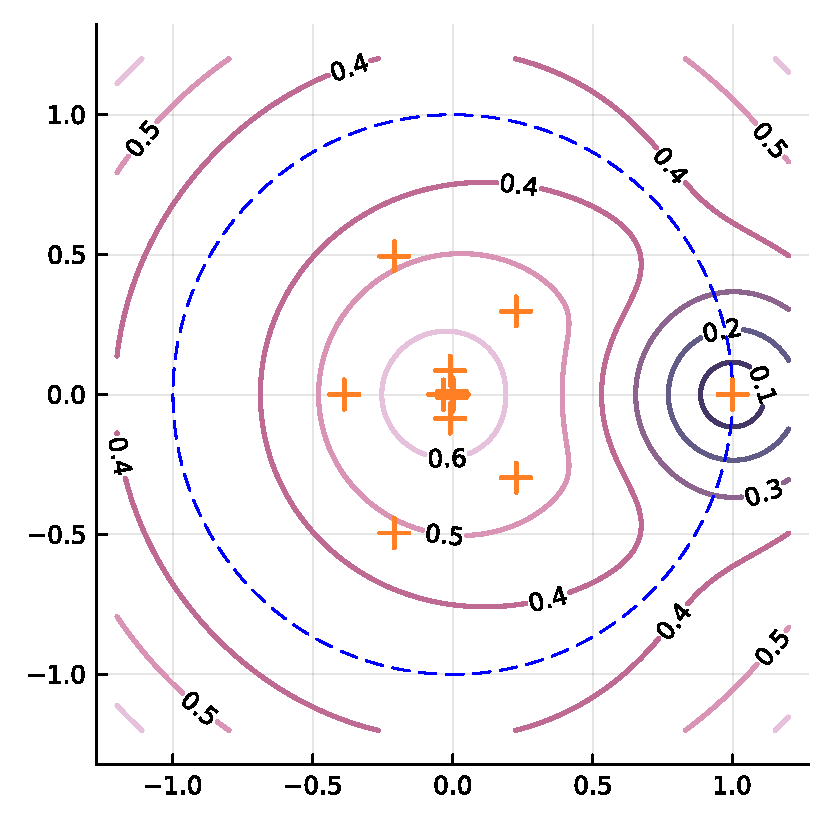
\includegraphics[width=0.5\textwidth]{resdmd.pdf}
    \caption{
        \todo{}
    }
\end{figure}


\subsection{kernel EDMD (kEDMD)}

\subsection{kernel ResDMD (kResDMD)}

% -------------------------------------------------------------------------------------- %
